\section{Ожидаемые технико-экономические показатели}

\subsection{Сокращение трудоемкости подготовки данных}

Выбранное техническое решение позволяет исключить промежуточный этап
формирования табличных файлов в формате \texttt{tbl/csv} \srcref{4} с
последующей
конвертацией в целевой формат хранения. За счет прямой генерации данных в
поддерживаемые колонoчные форматы \texttt{Parquet} \srcref{5},
\texttt{ORC} \srcref{6}, \texttt{Lance} \srcref{8} и \texttt{Vortex}
\srcref{9} сокращается количество операций, выполняемых при подготовке наборов
данных к нагрузочным испытаниям и исследовательским экспериментам.
Детерминированный характер генерации, предусмотренный спецификацией TPC-H
\srcref{1}, дополнительно упрощает повторное
проведение экспериментов при одинаковых параметрах запуска.

\subsection{Снижение инфраструктурных издержек}

Прямая запись результата в локальную файловую систему и в
\texttt{S3}-совместимые хранилища позволяет отказаться от отдельного конвейера
выгрузки, последующей конвертации и доставки данных в среду выполнения
аналитических запросов. Отсутствие обязательной материализации промежуточных
форматов уменьшает потребность во временном дисковом пространстве и снижает
накладные расходы на подготовку испытательной и исследовательской
инфраструктуры.

\subsection{Расширение вариантов интеграции}

Отделение модуля генерации от слоя сериализации позволяет
использовать программу как встраиваемый источник табличных данных. В этом
режиме таблицы \texttt{TPC-H} формируются непосредственно в оперативной
памяти и передаются потребителю без промежуточной записи на диск. Исходная
реализация генератора представлена в репозитории \texttt{Schengen}
\srcref{10}.

Такой способ интеграции реализован для СУБД DuckDB в отдельном расширении
\srcref{11}. Расширение регистрирует представления таблиц
\texttt{TPC-H}, а обращение к ним приводит к вызову табличной функции
\texttt{SCHENGEN\_SCAN}, получающей данные напрямую из генератора в виде
батчей Apache Arrow \srcref{3}.

\begin{center}
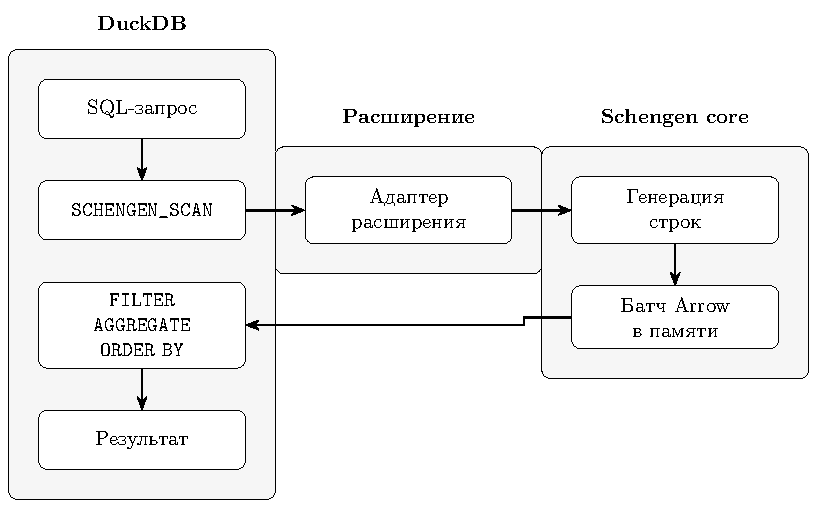
\includegraphics[width=0.78\textwidth]{image/duckdb-integration-diagram.pdf}
\captionof{figure}{Схема интеграции генератора с DuckDB}
\end{center}
\medskip

В листинге 5 приведен пример вывода \texttt{EXPLAIN} DuckDB для запроса
\texttt{TPC-H Q1} \srcref{1}. Наличие оператора \texttt{SCHENGEN\_SCAN} в нижней
части плана показывает, что данные поступают из генератора, а не считываются
из файла.

\begin{lstlisting}[style=duckdbplanlisting,caption={Вывод DuckDB \texttt{EXPLAIN} для запроса \texttt{TPC-H Q1}}]
D EXPLAIN SELECT
    l_returnflag,
    l_linestatus,
    SUM(l_quantity) AS sum_qty,
    SUM(l_extendedprice) AS sum_base_price,
    SUM(l_extendedprice * (1 - l_discount)) AS sum_disc_price,
    SUM(l_extendedprice * (1 - l_discount) * (1 + l_tax)) AS sum_charge,
    AVG(l_quantity) AS avg_qty,
    AVG(l_extendedprice) AS avg_price,
    AVG(l_discount) AS avg_disc,
    COUNT(*) AS count_order
FROM lineitem
WHERE l_shipdate <= DATE '1998-09-02'
GROUP BY l_returnflag, l_linestatus
ORDER BY l_returnflag, l_linestatus;

┌─────────────────────────────┐
│┌───────────────────────────┐│
││  Optimized Logical Plan   ││
│└───────────────────────────┘│
└─────────────────────────────┘
┌───────────────────────────┐
│          ORDER_BY         │
│    ────────────────────   │
│    "temp".main.lineitem   │
│       .l_returnflag       │
│    "temp".main.lineitem   │
│       .l_linestatus       │
└─────────────┬─────────────┘
┌─────────────┴─────────────┐
│         PROJECTION        │
│    ────────────────────   │
│        Expressions:       │
│        l_returnflag       │
│        l_linestatus       │
│          sum_qty          │
│       sum_base_price      │
│       sum_disc_price      │
│         sum_charge        │
│          avg_qty          │
│         avg_price         │
│          avg_disc         │
│        count_order        │
│                           │
│      ~1,199,999 rows      │
└─────────────┬─────────────┘
┌─────────────┴─────────────┐
│         AGGREGATE         │
│    ────────────────────   │
│          Groups:          │
│        l_returnflag       │
│        l_linestatus       │
│                           │
│        Expressions:       │
│      sum(l_quantity)      │
│    sum(l_extendedprice)   │
│          sum(#4)          │
│ sum((#4 * (1.0 + l_tax))) │
│      avg(l_quantity)      │
│    avg(l_extendedprice)   │
│      avg(l_discount)      │
│        count_star()       │
│                           │
│      ~1,199,999 rows      │
└─────────────┬─────────────┘
┌─────────────┴─────────────┐
│         PROJECTION        │
│    ────────────────────   │
│        Expressions:       │
│        l_returnflag       │
│        l_linestatus       │
│         l_quantity        │
│      l_extendedprice      │
│ (l_extendedprice * (1.0 - │
│        l_discount))       │
│           l_tax           │
│         l_discount        │
│                           │
│      ~1,200,000 rows      │
└─────────────┬─────────────┘
┌─────────────┴─────────────┐
│         PROJECTION        │
│    ────────────────────   │
│        Expressions:       │
│         l_quantity        │
│      l_extendedprice      │
│         l_discount        │
│           l_tax           │
│        l_returnflag       │
│        l_linestatus       │
│                           │
│      ~1,200,000 rows      │
└─────────────┬─────────────┘
┌─────────────┴─────────────┐
│           FILTER          │
│    ────────────────────   │
│        Expressions:       │
│ (l_shipdate <= '1998-09-02│
│          '::DATE)         │
│                           │
│      ~1,200,000 rows      │
└─────────────┬─────────────┘
┌─────────────┴─────────────┐
│       SCHENGEN_SCAN       │
│    ────────────────────   │
│      ~6,000,000 rows      │
└───────────────────────────┘
\end{lstlisting}

\subsection{Ожидаемые оперативные показатели}

К ожидаемым оперативным показателям относятся воспроизводимость набора данных
при одинаковых параметрах запуска, возможность параллельной генерации таблиц
и партиций, поддержка генерации на больших значениях масштаба, а также прямая
запись результата в современные колонoчные форматы хранения и удаленные
\texttt{S3}-совместимые хранилища. Совокупность указанных свойств обеспечивает
пригодность программы для нагрузочных испытаний, сравнительного анализа
аналитических СУБД \srcref{2} и встраивания в исследовательские конвейеры
обработки данных.
